\section{Results}
\label{sec:results}

\subsection{Static results}
\label{sec:results_static}

The static evidence is best read in three layers. The small proxy benchmark only verifies that energy and force errors can be reported reproducibly across regime-aware splits. OpenREACT then exposes a clear energy--force tradeoff between charge-aware variants. Finally, the two public force-labeled surrogate systems show that charge-aware effects are real, but not reducible to a single universal ordering.

Two points matter for interpretation. First, the static task here is not a generic leaderboard exercise in which lower energy and force errors are interchangeable. For the present materials question, energy errors primarily affect relative ranking across structures and compression states, whereas force errors affect how the potential steers trajectories once the system is already moving away from a local basin.

Second, the surrogate systems should not be forced into a monotone narrative. If one public surrogate favors charge-aware fitting overall while another redistributes the gain between energy and force, that discrepancy is evidence about the scope of the method rather than noise in the benchmark.

On OpenREACT, the current \texttt{static\_charge} reference remains better on energy metrics, with test energy MAE $34.98 \pm 0.69$ and energy MSE $1265.97 \pm 54.73$, whereas the stabilized \texttt{self\_consistent} branch reaches $35.65 \pm 1.07$ and $1318.73 \pm 83.30$. The ranking reverses on force MAE: \texttt{self\_consistent} improves from $3.53 \times 10^{-2} \pm 4.64 \times 10^{-3}$ to $3.25 \times 10^{-2} \pm 2.49 \times 10^{-3}$. OpenREACT therefore already shows that self-consistency is active without being uniformly superior: the static-charge approximation remains more favorable on energy aggregation, whereas the self-consistent branch improves force accuracy.

Transition1x gives a cleaner static ordering. In the matched multiseed comparison over seeds $7$ and $123$, \texttt{static\_charge} is strongest overall, reaching energy MAE $0.1232 \pm 0.0841$, energy MSE $0.0265 \pm 0.0292$, and force MAE $0.1946 \pm 0.0429$. The \texttt{self\_consistent} family remains clearly better than \texttt{short\_range}, but it does not surpass \texttt{static\_charge}: it reaches $0.1515 \pm 0.0392$, $0.0329 \pm 0.0159$, and $0.2164 \pm 0.0180$, while \texttt{short\_range} remains weakest at $0.1784 \pm 0.0288$, $0.0463 \pm 0.0108$, and $0.2214 \pm 0.0070$.

This is the strongest positive static result on the public surrogates. Transition1x is the first system in this study on which the charge-aware families do not merely trade one observable against another; instead, they outperform the short-range baseline across the full static metric set, even though the internal ordering between \texttt{static\_charge} and \texttt{self\_consistent} remains unresolved. It therefore supports the scientific relevance of charge-aware modelling more strongly than it supports the fully self-consistent branch as a final endpoint.

SPICE provides the clearest counterexample. In the matched multiseed comparison, \texttt{short\_range} is strongest on energy metrics, with energy MAE $173.84 \pm 2.25$ and energy MSE $41523.66 \pm 2809.30$. Both charge-aware branches remain better on force MAE, however: \texttt{static\_charge} reaches $0.01126 \pm 0.00218$ and \texttt{self\_consistent} reaches $0.01131 \pm 0.00265$, versus $0.01354 \pm 0.00172$ for \texttt{short\_range}.

The static ordering is therefore not only dataset-dependent, but different in exactly the way that matters for the final claim: one public surrogate system favors charge-aware families overall, while the other favors \texttt{short\_range} on energy and charge-aware families on force.

SPICE is valuable precisely because it resists a cleaner headline. If Transition1x were the only surrogate system, the favorable charge-aware ordering could still be dismissed as a peculiarity of one chemical manifold. By contrast, SPICE shows that the electrostatic correction remains active but reallocates its benefit: the short-range baseline recovers the best energy statistics, whereas the charge-aware branches retain the best force MAE. For the present argument, that heterogeneity is more informative than a false appearance of universality.

The final CL-20/HMX benchmark now provides the decisive static test. In the matched multiseed comparison over seeds $42$ and $123$, the ordering is cleaner than on either public surrogate: \texttt{self\_consistent} reaches energy MAE $397.37 \pm 88.41$ and energy MSE $1.83 \times 10^{5} \pm 7.11 \times 10^{4}$, followed by \texttt{static\_charge} at $419.26 \pm 54.34$ and $2.02 \times 10^{5} \pm 3.79 \times 10^{4}$, whereas \texttt{short\_range} remains weakest at $479.24 \pm 94.83$ and $2.64 \times 10^{5} \pm 8.84 \times 10^{4}$. Force MAE is effectively tied across the three families at $1.72347$.

The charge diagnostics show that the two electrostatic branches are not numerically inert on this target: both maintain neutrality residuals at numerical precision ($\sim 5 \times 10^{-9}$), while \texttt{self\_consistent} sustains a slightly stronger charge and field response than \texttt{static\_charge} (test charge RMS $7.72 \times 10^{-3}$ vs.\ $7.44 \times 10^{-3}$; field RMS $1.67 \times 10^{-3}$ vs.\ $1.56 \times 10^{-3}$). The associated supporting QEq table is included with the submission specifically to show that the electrostatic branches remain measurably active on the final target rather than acting as a numerically inert correction.

A regenerated material-specific held-out table sharpens the split interpretation: under the original deterministic contiguous split, the test segment is HMX-only, and on that held-out HMX slice the same family ordering persists (\texttt{self\_consistent} best, \texttt{static\_charge} second, \texttt{short\_range} weakest). More importantly, the cleaner material-balanced CL-20/HMX split-v2 evaluation preserves the same static hierarchy on a jointly held-out material mix: \texttt{self\_consistent} reaches test energy MAE $22704.77$, \texttt{static\_charge} reaches $23026.01$, and \texttt{short\_range} reaches $23557.23$, while force MAE remains effectively tied at $1.91821$.

The cleaner held-out evaluation is numerically harsher than the earlier contiguous slice, but it resolves the key reviewer concern in the favorable direction: the final-target static ordering is not an artifact of the original HMX-only test segment. The real energetic-material target therefore resolves the public-target heterogeneity in a specific direction even after split cleanup: charge-aware modeling materially improves the static energy hierarchy, and the fully self-consistent branch remains the strongest static family on the final benchmark.

Taken together, the static evidence supports a sharper conclusion than the public data alone. Charge-aware response is physically meaningful across all benchmark tiers, but only the final CL-20/HMX target makes the preferred static ordering unambiguous. On that target, the remaining question is not whether electrostatic response matters, but whether the associated static gain can be transferred to nonequilibrium dynamics without incurring a new stability cost.

\begin{figure}[t]
    \centering
    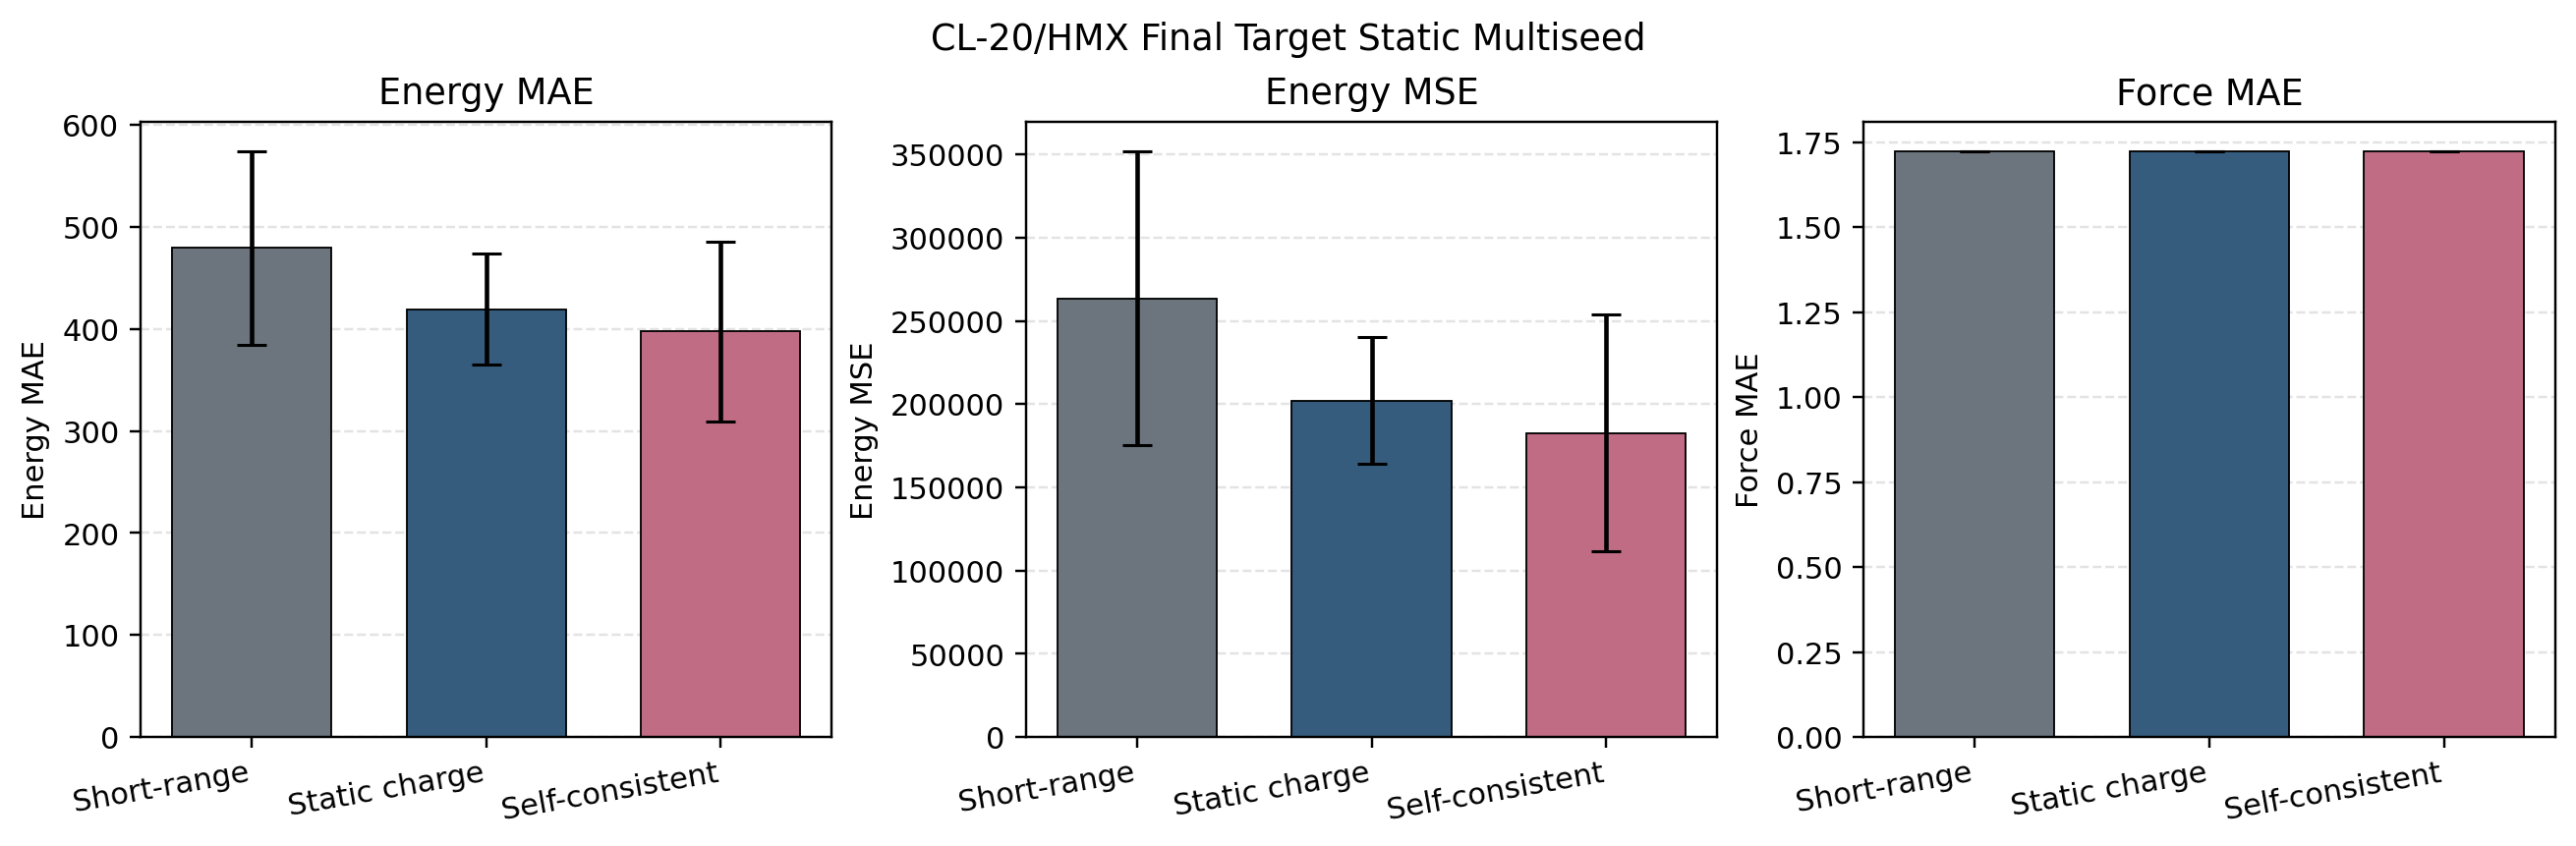
\includegraphics[width=0.92\linewidth]{figs/cl20_hmx_target_static_multiseed.png}
    \caption{CL-20/HMX final-target static multiseed comparison over seeds $42$ and $123$. The energy hierarchy is unambiguous on the energetic-material target: \texttt{self\_consistent} is best, \texttt{static\_charge} is second, and \texttt{short\_range} is weakest, while force MAE remains effectively tied.}
    \label{fig:cl20_hmx_target_static_multiseed}
\end{figure}

\begin{figure}[t]
    \centering
    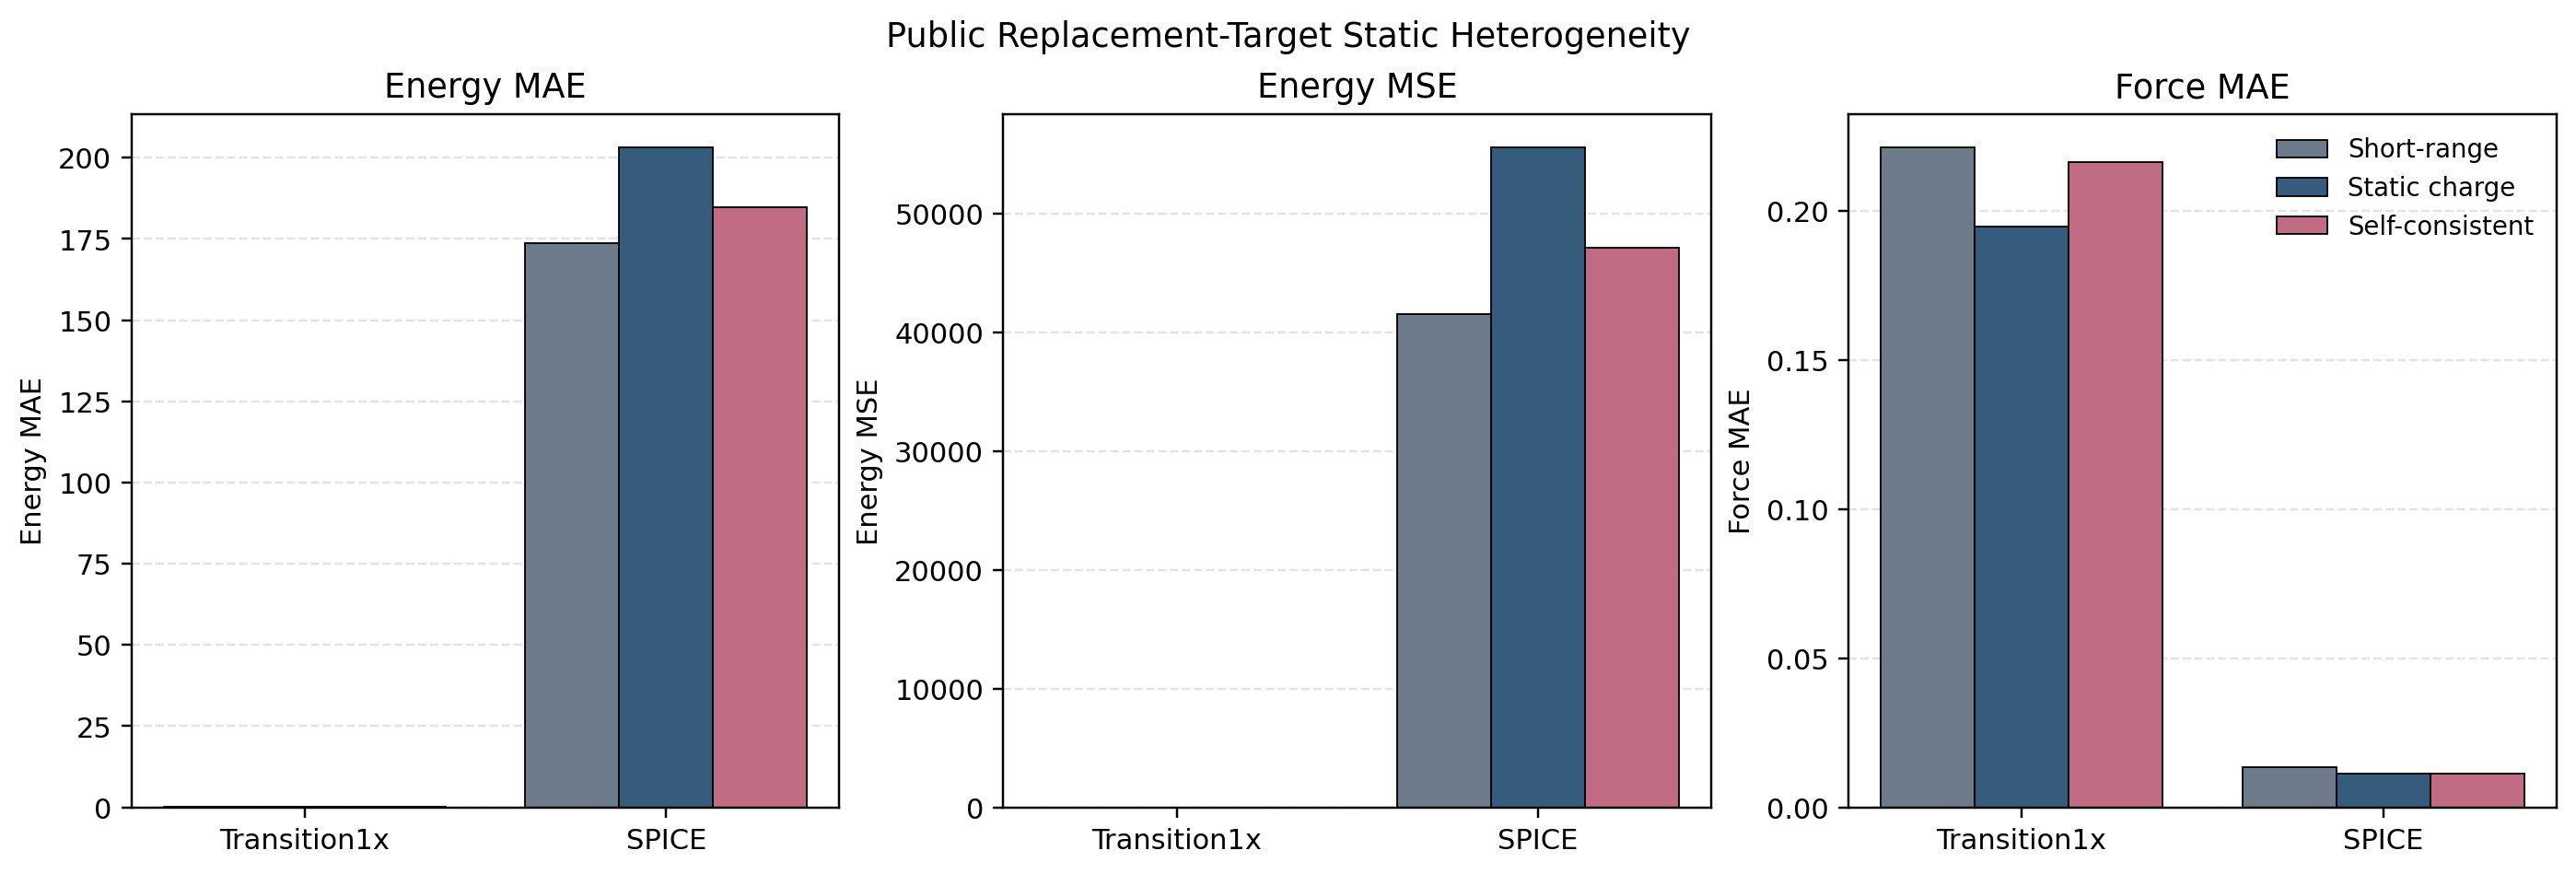
\includegraphics[width=\linewidth]{figs/replacement_target_static_summary.png}
    \caption{Static heterogeneity across the two public surrogate systems. Transition1x favors the charge-aware families overall, whereas SPICE favors \texttt{short\_range} on energy metrics but the charge-aware branches on force MAE.}
    \label{fig:replacement_target_static_summary}
\end{figure}

\begin{figure}[t]
    \centering
    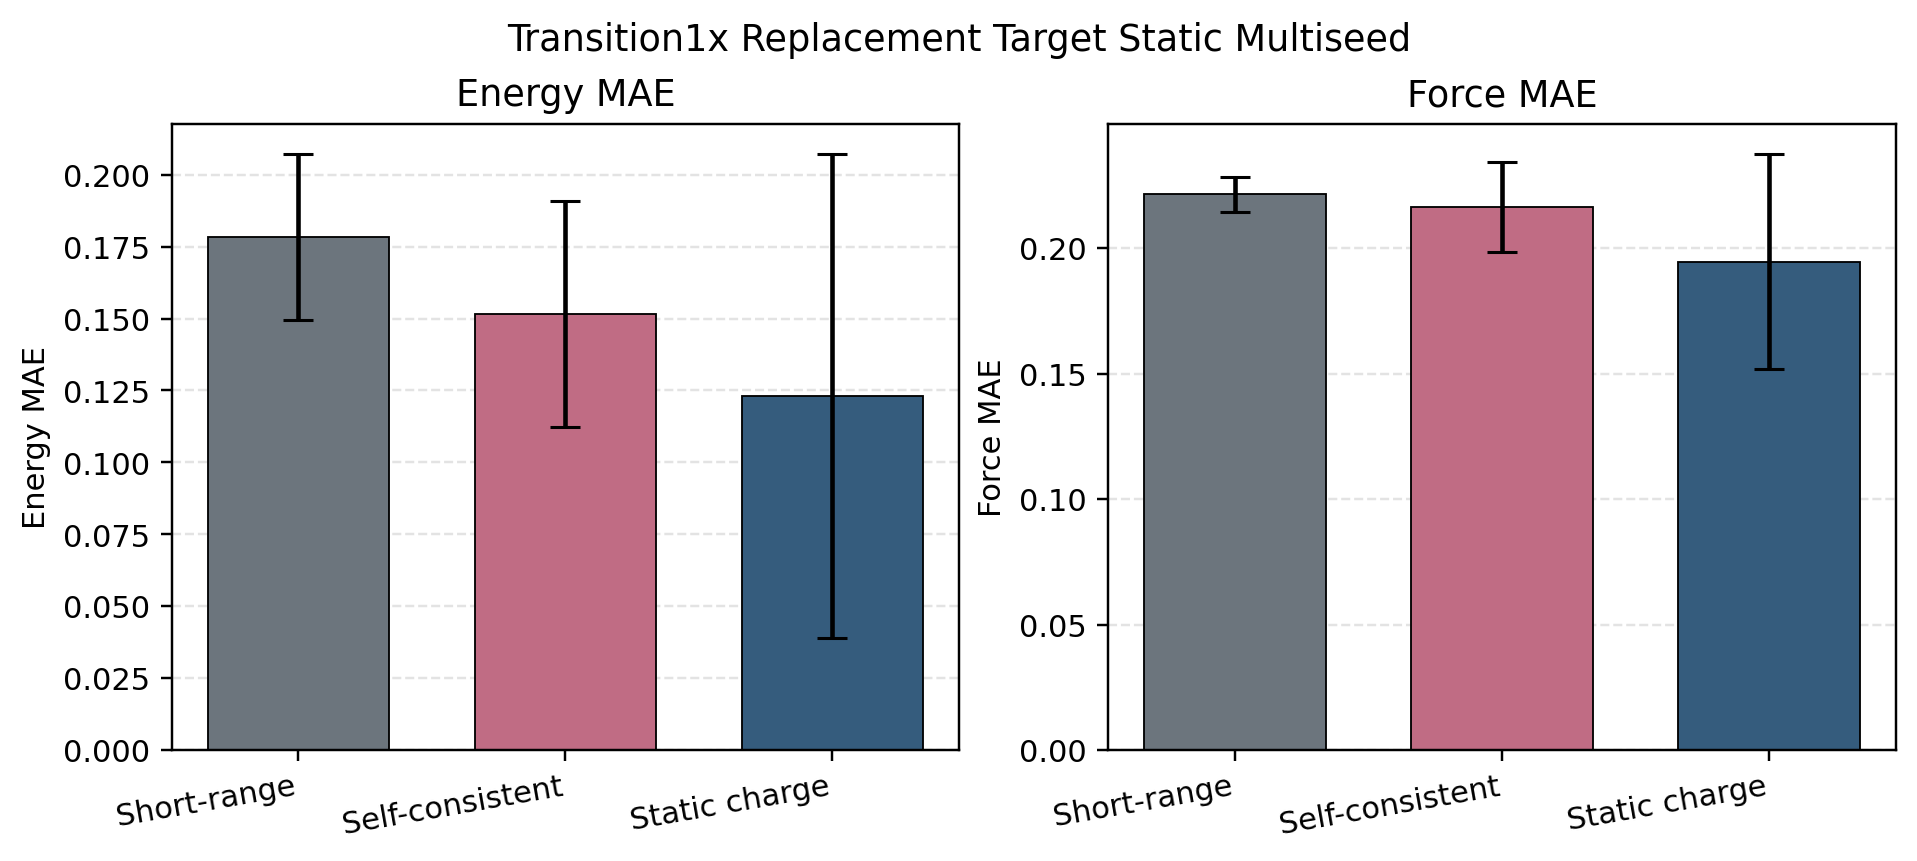
\includegraphics[width=0.92\linewidth]{figs/transition1x_target_static_multiseed.png}
    \caption{Transition1x static multiseed comparison over seeds $7$ and $123$. Both charge-aware variants outperform the short-range baseline, and \texttt{static\_charge} is the strongest overall family.}
    \label{fig:transition1x_target_static_multiseed}
\end{figure}

\begin{figure}[t]
    \centering
    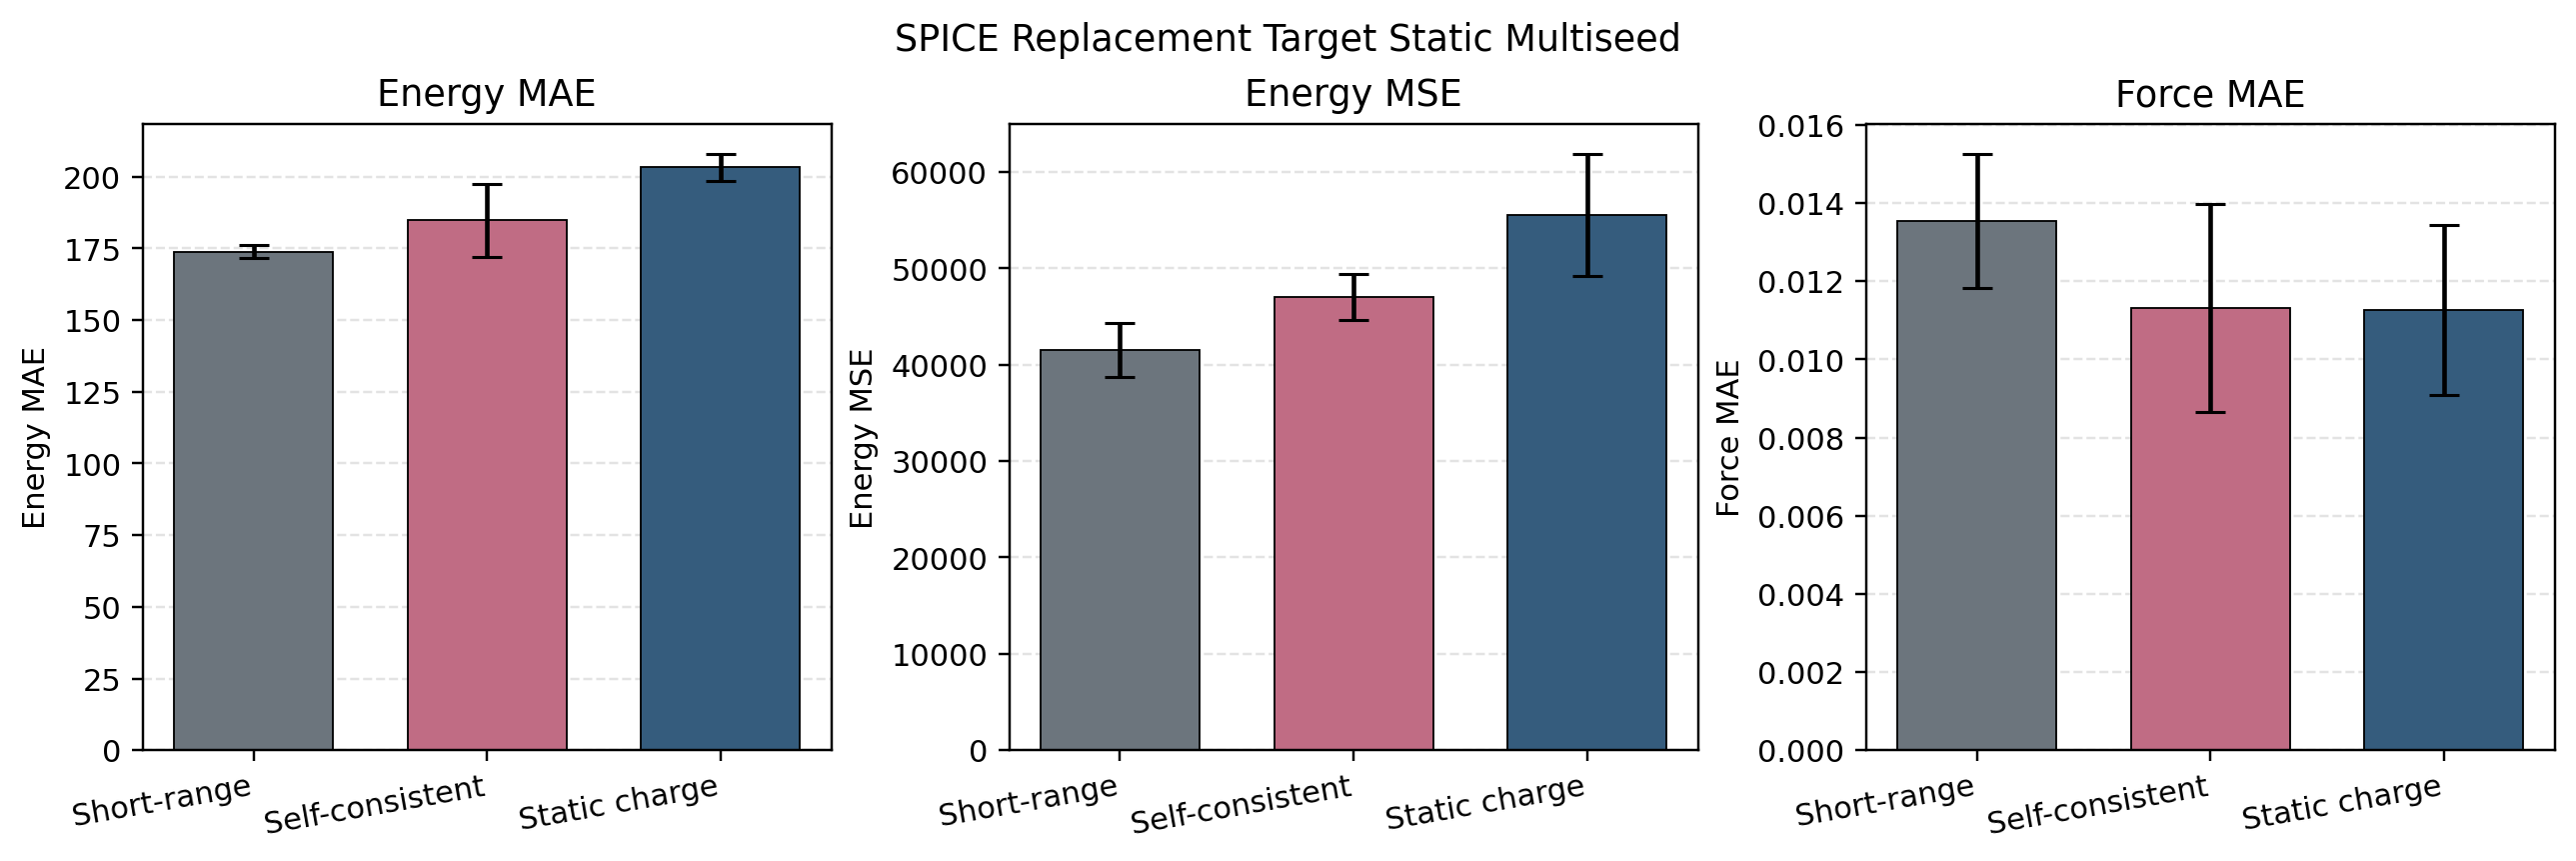
\includegraphics[width=0.92\linewidth]{figs/spice_target_static_multiseed.png}
    \caption{SPICE static multiseed comparison over seeds $7$ and $123$. \texttt{short\_range} is strongest on energy metrics, whereas both charge-aware branches improve force MAE and remain nearly tied.}
    \label{fig:spice_target_static_multiseed}
\end{figure}

\begin{figure}[t]
    \centering
    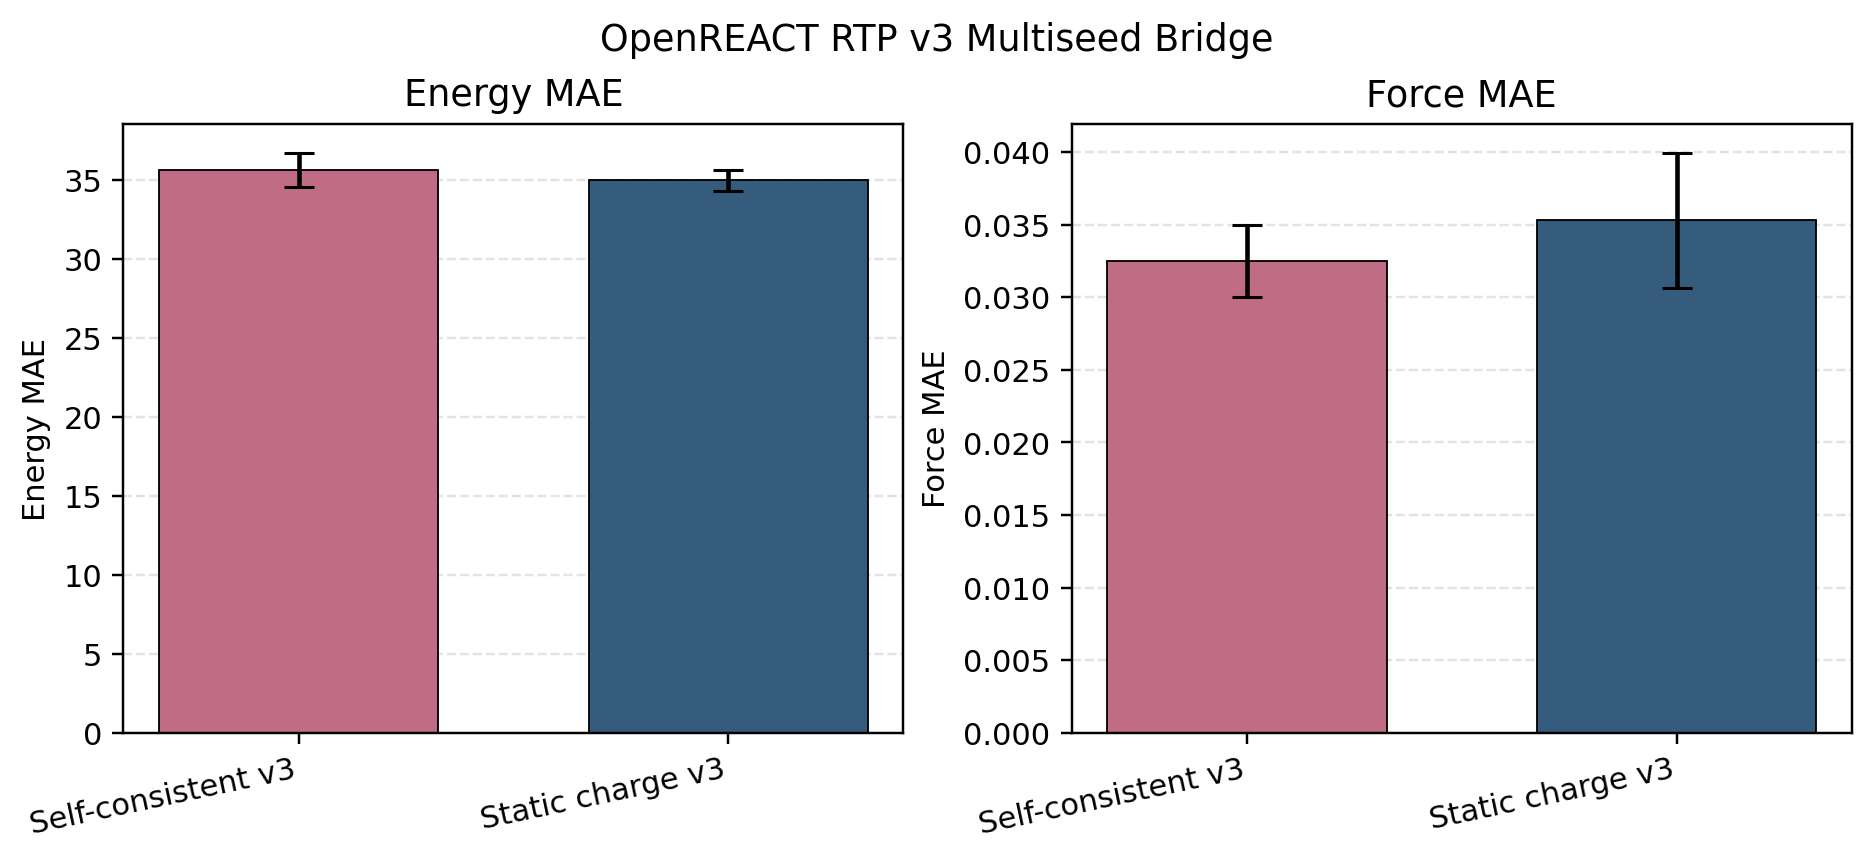
\includegraphics[width=0.92\linewidth]{figs/openreact_v3_multiseed_static.png}
    \caption{OpenREACT public reference system, conservative v3 multiseed comparison over seeds $7$ and $123$. The static-charge reference remains better on energy MAE, while the stabilized self-consistent branch improves force MAE.}
    \label{fig:openreact_v3_static}
\end{figure}
